\documentclass[10pt,aspectratio=169,serif]{beamer}

\usepackage[fontset=none, scheme=plain]{ctex}
\IfFontExistsTF{Songti SC}{%
	\setCJKmainfont{Songti SC}[AutoFakeSlant=0.2]%
	\setCJKsansfont{Songti SC}[AutoFakeSlant=0.2]%
}{%
	\setCJKmainfont{FandolSong-Regular}[Extension=.otf,BoldFont=FandolSong-Bold,AutoFakeSlant=0.2]%
	\setCJKsansfont{FandolSong-Regular}[Extension=.otf,BoldFont=FandolSong-Bold]%
}
\usepackage{amsmath,amssymb,graphicx,tikz,booktabs,multicol,calligra}
\usepackage{pgfplots}
\pgfplotsset{compat=1.18}
\usepackage{tcolorbox}
\tcbuselibrary{skins}
\usepackage{XyygU}
\usepackage{caption}
\captionsetup[figure]{name=图,labelsep=period}

\usetikzlibrary{arrows.meta,positioning,calc}

\setlength{\abovedisplayskip}{0pt plus 2pt minus 2pt}
\setlength{\belowdisplayskip}{0pt plus 2pt minus 2pt}

\title[4.1 指数 练习]{4.1 指数（课后练习）}
\subtitle{实数指数幂及其运算性质}
\author{}
\institute{}
\date{2026-10-16}

\begin{document}

\begin{frame}
  \titlepage
\end{frame}

% ========== 第1题 ==========
\begin{frame}[t]{第1题：计算实数指数幂}
\textbf{1.} 计算下列各式：
\[
(1)\ \left(2^{\sqrt{3}}\sqrt{m^{\sqrt{3}}}\right)^{2\sqrt{3}};\qquad
(2)\ a^{\frac{\pi}{3}}a^{\frac{2\pi}{3}}a^{-\pi}.
\]
\end{frame}

\begin{frame}[t]{第1题 解答}
\begin{tcolorbox}[colback=orange!10,colframe=orange,title=\textbf{解}]
\textbf{(1)} 先把根式写成分数指数幂：$\sqrt{m^{\sqrt{3}}}=m^{\frac{\sqrt{3}}{2}}$，
再利用 $(a^{r}a^{s})^{t}=a^{rt}a^{st}$：
\[
\left(2^{\sqrt{3}}\,m^{\frac{\sqrt{3}}{2}}\right)^{2\sqrt{3}}
= \bigl(2^{\sqrt{3}}\bigr)^{2\sqrt{3}}\cdot\bigl(m^{\frac{\sqrt{3}}{2}}\bigr)^{2\sqrt{3}}
= 2^{(\sqrt{3})(2\sqrt{3})}\cdot m^{\frac{\sqrt{3}}{2}\cdot 2\sqrt{3}}.
\]
\[
= 2^{6}\cdot m^{3} = 64\,m^{3}.
\]

\vspace{0.6em}
\textbf{(2)} 利用 $a^{r}a^{s}=a^{r+s}$ 把指数相加：
\[
a^{\frac{\pi}{3}+\frac{2\pi}{3}-\pi} = a^{\pi-\pi} = a^{0} = 1.
\]
\end{tcolorbox}
\end{frame}

% ========== 第2题 ==========
\begin{frame}[t]{第2题：探究实数指数幂的变化趋势}
\textbf{2.} 利用计算工具，探究下列实数指数幂的变化规律：

(1) $x$ 取负实数，使得 $|x|$ 的值逐渐增大并趋向于无穷大，计算相应的 $2^{x}\ (x\in\mathbf{R})$ 的值，观察变化趋势；

(2) $x$ 取正实数，使得 $x$ 的值逐渐增大并趋向于无穷大，计算相应的 $\left(\dfrac{1}{2}\right)^{x}\ (x\in\mathbf{R})$ 的值，观察变化趋势。
\end{frame}

\begin{frame}[t]{}\vspace{-1em}
\begin{tcolorbox}[colback=orange!10,colframe=orange,title=\textbf{解}]
\textbf{(1)} 列表观察：
\[
\begin{array}{c|cccccc}
x & -1 & -2 & -5 & -10 & -20 & \cdots\\ \hline
2^{x}=2^{-|x|}\rule[8pt]{0pt}{5pt} & 0.5 & 0.25 & 0.03125 & \approx 0.00098 & \approx 9.5\times 10^{-7} & \to 0
\end{array}
\]
当 $x<0$ 且 $|x|\to +\infty$ 时，$2^{x}=2^{-|x|}=\left(\frac{1}{2}\right)^{|x|}\to 0$。

\vspace{0.6em}
\textbf{(2)} 列表观察：
\[
\begin{array}{c|cccccc}
x & 1 & 2 & 5 & 10 & 20 & \cdots\\ \hline
\left(\frac{1}{2}\right)^{x}\rule[10pt]{0pt}{5pt} & 0.5 & 0.25 & 0.03125 & \approx 0.00098 & \approx 9.5\times 10^{-7} & \to 0
\end{array}
\]
当 $x>0$ 且 $x\to +\infty$ 时，$\left(\frac{1}{2}\right)^{x}\to 0$。

\vspace{0.6em}
\textbf{结论：} 两个式子都随着自变量绝对值的增大而无限趋近于 $0$。
\end{tcolorbox}
\end{frame}

\begin{frame}[t]{第2题 图象示意}
\begin{center}
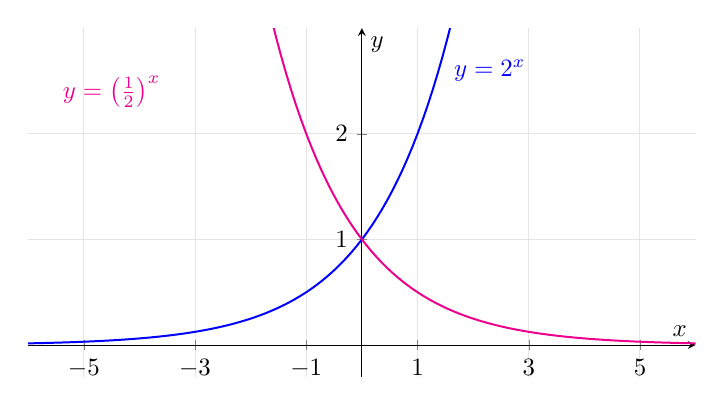
\begin{tikzpicture}[scale=0.9]
\begin{axis}[
    width=11cm, height=6.5cm,
    axis lines=middle,
    xlabel=$x$, ylabel=$y$,
    xmin=-6, xmax=6, ymin=-0.3, ymax=3,
    xtick={-5,-3,-1,1,3,5},
    ytick={0,1,2},
    grid=major, grid style={gray!20},
]
\addplot[thick,blue,domain=-6:3,samples=100] {2^x};
\addplot[thick,magenta,domain=-3:6,samples=100] {0.5^x};
\node[blue] at (axis cs:2.3,2.6) {$y=2^{x}$};
\node[magenta] at (axis cs:-4.5,2.4) {$y=\left(\frac{1}{2}\right)^{x}$};
\end{axis}
\end{tikzpicture}
\end{center}
\end{frame}

\begin{frame}[c]
  \begin{center}
    {\Huge\calligra Thanks!}
  \end{center}
\end{frame}

\end{document}
